%%%%%%%%%%%%%%%%%%%%%%%%%%%%%%%%%%%%%%%%%%%%%%%%%%%%%%%%%%%%%%%%%%%%%%%%%%%%%%%%%%%%%%%%%%%%%%%%
% Differential
%%%%%%%%%%%%%%%%%%%%%%%%%%%%%%%%%%%%%%%%%%%%%%%%%%%%%%%%%%%%%%%%%%%%%%%%%%%%%%%%%%%%%%%%%%%%%%%%
\section{Differentialrechnung\formelbuchyellow{443}}
	$ f'(x_0) = \frac{df}{dx}\left|_{x=x_0}\right. = (\frac{d}{dx}f)_{x=x_0} = Df(x_0) = \lim\limits_{h \rightarrow 0} \frac{f(x_0+h) - f(x_0)}{h} = \lim\limits_{h \rightarrow 0} \frac{\Delta f}{\Delta x}$ und $ (f^{-1})' = \frac{1}{f' \circ f^{-1}}$\\
	$f^{-1}$ ist differenzierbar wenn: $f$ differenzierbar und umkehrbar ist und wenn $f'(x) \neq 0$ ist. \\
	Rechtsseitige $f_{r}'(x_0)$ bzw. linksseitige $f_{l}'(x_0)$ Ableitung.\\
	Falls $f_{r}'(x_0) = f_{l}'(x_0)$ und $f$ an der Stelle $x_0$ stetig, dann ist $f$ an der Stelle $x_0$ differenzierbar. 

\subsection{Ableitungsregeln\formelbuchyellow{449}}

\subsection{Einige Ableitungen\formelbuchyellow{445}}
	\begin{minipage}[t]{6cm} 		
		$(|x|)' = sgn(x) = \frac{|x|}{x} = \frac{x}{|x|}, x \neq 0$\\
		$\ln(|x|)' = \frac{1}{x}$
	\end{minipage} 
	\begin{minipage}[t]{6.5cm} 		
		$(\tan x)' = 1 + \tan^2{ }x , x \in \mathbb{R}\backslash \left\{ \frac{2k+1}{2}\pi \right\} $\\
		$(\tanh x)' = 1 - \tanh^2 x$ 
	\end{minipage} 
	\begin{minipage}[t]{6cm} 		
		$(\cot x)' = -(1 + \cot^2{ }x) , x \in \mathbb{R}\backslash \left\{ k\pi \right\} $\\
		$(\coth x)' = 1 - \coth ^2 x$
	\end{minipage} 

\subsection{H"ohere Ableitungen\formelbuchyellow{451}}
	\begin{minipage}[t]{9.5cm} 
		$ (\sin x)^{(2k+1)} = (-1)^k \cos x, k \in \mathbb{N}_0 $ 
	\end{minipage} 
	\begin{minipage}[t]{9.5cm} 
		$ (\sin x)^{(2k)} = (-1)^k \sin x, k \in \mathbb{N} $
	\end{minipage} \\
	\begin{minipage}[t]{9.5cm} 
		$ (\cos x)^{(2k-1)} = (-1)^k \cos x, k \in \mathbb{N} $ 
	\end{minipage} 
	\begin{minipage}[t]{9.5cm} 
		$ (\cos x)^{(2k)} = (-1)^k \cos x, k \in \mathbb{N} $
	\end{minipage} \\
	\begin{minipage}[t]{9.5cm} 
		$ \left(\frac{1+x}{1-x}\right)^{(n)} = \frac{2 \cdot n!}{(1-x)^{n+1}} $
	\end{minipage} 
	\begin{minipage}[t]{9.5cm} 
		$ (\sqrt{x})^{(n)} = (-1)^{n+1} \cdot \frac{1 \cdot 3 \cdot ... \cdot (2n-3)}{2^n x^{n-1} \sqrt{x}} $
	\end{minipage}  \\
	\begin{minipage}[t]{9.5cm} 
		$ \left(ln\frac{1+x}{1-x}\right)^{(n)} = (-1)^{n+1} \cdot \frac{(n-1)!}{(1+x)^n} + \frac{(n-1)!}{(1-x)^n}$
	\end{minipage} 
	\begin{minipage}[t]{9.5cm} 
		$ (x \cdot e^{x})^{(n)} = n \cdot e^x + x \cdot e^x = e^x (n + x)$
	\end{minipage} 
	
\subsection{Tangentengleichung}
	$\hat{f}(x) = \underbrace{\overbrace{(x - x_0)}^{dx} \cdot f'(x_0)}_{dy} + f(x_0) \qquad (x_0 = $Entwicklungspunkt$)$ 

\subsection{Differential, Fehlerrechnung\formelbuchyellow{865}} 
	\begin{minipage}[c]{7cm} 
		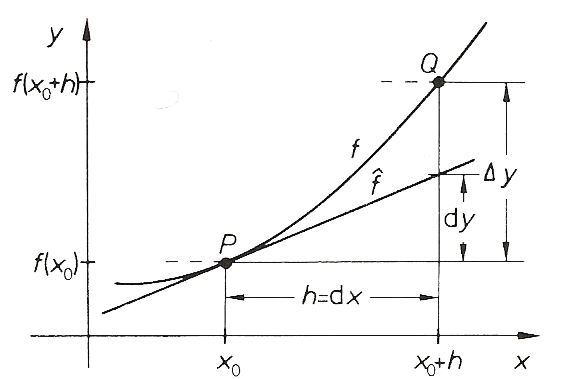
\includegraphics[width=5cm]{./bilder/differential_fehlerrechnung.png} 
	\end{minipage}
	\begin{minipage}[c]{13cm} 
		absoluter Fehler: $\left| \Delta y \right|	\approx \left| dy \right|=\left|f'(\bar{x})\right|\cdot\left| dx \right| \leq	\left| f'(\bar{x}) \right| \cdot \left| \delta \right| $  \\
		relativer Fehler: $|\Delta y| \approx |\frac{dy}{y}| = |\frac{f'(x)}{y}| \cdot |dx| \leq |\frac{f'(x)}{y}| \cdot |\delta| = |\frac{f'(x)}{f(x)} \cdot |\delta|  $ \\
		$|\frac{dx}{x}| \hat{=}$relative Fehler Input$ \qquad |\frac{dy}{y}| \hat{=} $relative Fehler Output$ \qquad $Einheit$ = [1]$\\
		Auf n-Stellen nach dem Komma genau $\Rightarrow \mbox{absoluter Fehler: } \delta = \pm 0.5 \cdot 10^{-n}$ 
	\end{minipage}


\subsection{Mittelwertsatz\formelbuchyellow{453}}
	\begin{minipage}[c]{5cm} 
		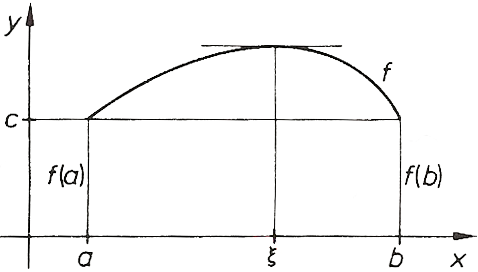
\includegraphics[width=3cm]{./bilder/differential_mittelwertsatz.png} 
	\end{minipage}
	\begin{minipage}[c]{7cm} 
		$\frac{\Delta y}{\Delta x}=\frac{f(b) - f(a)}{b - a} = f'(\xi) $ \\
		$\xi = a + \delta(b-a)$
	\end{minipage}
	\begin{minipage}[c]{5cm}
		$\frac{f(x+h) - f(x)}{h} = f'(x+\delta h)$\\
		$f(x+h) = h \cdot f'f(x+\delta h) + f(x)$ \\
		$\xi = x + \delta h \qquad 0<\delta<1$
	\end{minipage}	

\subsection{Taylor Polynom\formelbuchyellow{454,483}}
	($x_0$ = Entwicklungspunkt)$\quad f(x_0+h)=f(x_0) + f'(x_0)h + \frac{f''(x_0)}{2}h^2 + \frac{f'''(x_0)}{3!}h^3 + \ldots + \frac{f^{(n)}(x_0)}{n!}h^n + R_n(x_0, h)$\\
	$ h = x-x_0$\\
	$R_n$(Lagrange):$\quad R_n(x_0, h) = \frac{f^{(n+1)}(x_0 + \delta h)}{(n+1)!}h^{n+1}, (0 < \delta < 1);
	\qquad 
	\lim_{n \to \infty} R_n(x_0, h) = 0 \Longrightarrow f(x_0+h) = \sum\limits_{n=0}^{\infty} \frac{f^{(n)}(x_0)}{n!}h^n$\\	
	\flushleft MacLaurinsche-Form (gilt f"ur $x_0=0, h=x $): $ f(x)=\sum\limits_{k=0}^{n} \frac{f^{(k)}(0)}{k!} \cdot x^k + R_n; 
	\qquad 
	R_n = \frac{f^{(n+1)}(\delta x)}{(n+1)!} \cdot x^{n+1}, (0 < \delta < 1);$
	
\subsubsection{Einige Reihen\formelbuchyellow{19,476,1073}}
		$\sin x = x - \frac{x^3}{3!} +  \frac{x^5}{5!} \mp ... + (-1)^{n-1} \cdot \frac{x^{2n-1}}{(2n-1)!} + $
		$ \overbrace{(-1)^n \cdot \frac{\cos(\vartheta x)}{(2n+1)!} \cdot x^{2n+1}}^{R_n} $\\
		$e^x =  1 + \frac{x}{1} + \frac{x^2}{2!} + ... + \frac{x^n}{n!} + $
		$ \frac{e^{\vartheta x}}{(n+1)!} \cdot x^{n+1} $\\
		$\ln (1+x) = x - \frac{x^2}{2} + \frac{x^3}{3} \mp ... + (-1)^{n-1} \cdot \frac{x^n}{n} + $
		$ \frac{(-1)^n}{(1+\vartheta x)^{n+1}} \cdot \frac{x^{n+1}}{n+1} $ 

\subsection{Bernoulli-de l'Hospital\formelbuchyellow{56}}
	${lim} _{x\downarrow x_{0}} \frac{f_{1}(x)}{f_{2}(x)} = {lim} _{x\downarrow x_{0}} \frac{f'_{1}(x)}{f'_{2}(x)} $, dies gilt f"ur: "`$\frac{0}{0}$"' 1. Regel, oder "`$\frac{\pm\infty}{\pm\infty}$"' 2. Regel;   Z"ahler und Nenner separat ableiten!

\subsubsection{Spezialf"alle}
	\begin{minipage}[c]{7cm} 
		$0 \cdot \pm \infty$ $\Rightarrow$ $\frac{f_1}{\frac{1}{f_2}} = \frac{0}{0}$ oder $\frac{f_2}{\frac{1}{f_1}} = \frac{\pm \infty}{\pm \infty}$
	\end{minipage}
	\begin{minipage}[c]{4cm} 
		$\infty - \infty$ $\Rightarrow$ $\frac{\frac{1}{f_2} - \frac{1}{f_1}}{\frac{1}{f_1 \cdot f_2}} $
	\end{minipage}
	\begin{minipage}[c]{7cm} 
		$ f^g:
		\left\{ 	
			\begin{array}{l} 
				1^\infty \\ 
				0^0 \\ 
				\infty^0 
			\end{array} 
		\right\} =
	  e^{g \cdot ln(f)} =
		\left\{ 
			\begin{array}{l} 
				e^{\infty \cdot 0} \\ 
				e^{0 \cdot -\infty} \\ 
				e^{0 \cdot \infty}
			\end{array}
		\right\} $
	\end{minipage}	

\subsection{Kurvenuntersuchungen\formelbuchyellow{260}}
\begin{enumerate}
	\item Definitionsbereich\formelbuchyellow{48} $D_f$ und Absch"atzung des Wertebereichs $W_f$, wenn m"oglich anhand der Extremalstellen
	\item Symmetrie und Periodizit"at\formelbuchyellow{52}
	\item Nullstellen
	\item Stetigkeit\formelbuchyellow{59} und Differenzierbarkeit\formelbuchyellow{443} (Berechnung der Ableitungen)
	\item Extremwerte, Wendepunkte und Wendetangenten, Monotonie, Kr"ummungsverhalten\formelbuchyellow{51}
	\item Grenzwertaussagen (Asymptote, Pole, Verhalten von $f$ am Rande des Definitionsbereichs)
\end{enumerate}

\subsubsection{Monotonie\formelbuchyellow{452}}
\begin{tabular}{|c|c|c|c|c|l|}
	\hline $f'(x)$ & $f''(x)$ & $f'''(x)$ & $f^{(n-1)}(x)$ & $f^{(n)}$ & Funktion $f$ \\
	\hline $\geq 0$ & & & & & monoton wachsend\\
	\hline $> 0$ & & & & & streng monoton wachsend\\
	\hline $\leq 0$ & & & & & monoton fallend \\
	\hline $< 0$ & & & & & streng monoton fallend\\
	\hline $= 0$ & $= 0$ & $= 0$ & $\dots = 0$ & $> 0$ & streng monoton wachsend (falls $n$ ungerade)\\
	\hline $= 0$ & $= 0$ & $= 0$ & $\dots = 0$ & $< 0$ & streng monoton falls (falls $n$ ungerade) \\\hline
\end{tabular}

\subsubsection{Extremstelle\formelbuchyellow{455}}
\begin{tabular}{|c|c|c|c|c|l|}
	\hline $f'(x)$ & $f''(x)$ & $f'''(x)$ & $f^{(n-1)}(x)$ & $f^{(n)}$ & Funktion $f$ \\
	\hline $= 0$ & $> 0$ & & & & relatives Minimum, \textbf{Randstellen beachten}\\
	\hline $= 0$ & $< 0$ & & & & relatives Maximum, \textbf{Randstellen beachten}\\
	\hline $= 0$ & $= 0$ & $= 0$ & $\dots = 0$ & $> 0$ & relatives Minimum (falls $n$ gerade), \textbf{Randstellen beachten}\\
	\hline $= 0$ & $= 0$ & $= 0$ & $\dots = 0$ & $< 0$ & relatives Maximum (falls $n$ gerade), \textbf{Randstellen beachten}\\
	\hline\multicolumn{6}{|l|}{\textbf{Zweite Variante}  Falls bei $f'(x)$ an der Stelle $x_0$ ein Vorzeichenwechsel besteht, existiert dort eine Extremstelle} \\\hline
\end{tabular}

\subsubsection{Konvexit"at - Kr"ummungsverhalten\formelbuchyellow{253}}
\begin{tabular}{|c|c|c|c|c|l|}
	\hline $f'(x)$ & $f''(x)$ & $f'''(x)$ & $f^{(n-1)}(x)$ & $f^{(n)}$ & Funktion $f$ \\
	\hline & $\geq 0$ & & & & konvex (linksgekr"ummt)\\
	\hline & $> 0$ & & & & streng konvex (linksgekr"ummt)\\
	\hline & $\leq 0$ & & & & konkav (rechtsgekr"ummt)\\
	\hline & $< 0$ & & & & streng konkav (rechtsgekr"ummt)\\\hline
\end{tabular}

\subsubsection{Wendepunkte (Terassenpunkt)\formelbuchyellow{255}}
\begin{tabular}{|c|c|c|c|c|l|}
	\hline $f'(x)$ & $f''(x)$ & $f'''(x)$ & $f^{(n-1)}(x)$ & $f^{(n)}$ & Funktion $f$ \\
	\hline\ & $= 0$ & $\neq 0$ & & & Wendepunkt\\
	\hline $= 0$ & $= 0$ & $\neq 0$ & & & Terassen- oder Sattelpunkt\\
	\hline\multicolumn{6}{|l|}{\textbf{Zweite Variante}  Falls bei $f''(x)$ an der Stelle $x_0$ ein Vorzeichenwechsel besteht, existiert dort ein Wendepunkt} \\\hline
\end{tabular}

\subsubsection{Asymptote\formelbuchyellow{259}}
	Die Asymptote existiert nur wenn alle drei eigentlichen Grenzwerte existieren.
	F"ur Funktionen, die nicht gebrochenrational sind, kann die Asymptote wie folgt bestimmt werden. \\
	\ \\ %Leerzeile
 	Asymptote  $g: y = ax + b \Rightarrow \lim\limits_{x \rightarrow \infty}(f(x) - ax - b) = 0$\\
	\ \\ %Leerzeile
	$a = \lim\limits_{x \rightarrow \infty} \frac{f(x)}{x} $ oder $a = \lim\limits_{x \rightarrow \infty} f'(x) \qquad $\\
	gilt jedoch nur wenn in der ersten Formel die Bedingung f"ur Bernoulli-de l'Hospital erf"ullt sind.\\
	$b = \lim\limits_{x \rightarrow \infty} (f(x) - ax) $\\
	\ \\ %Leerzeile
	Dies alles gilt sinngem"ass auch f"ur $x \rightarrow -\infty$\\
	\ \\ %Leerzeile	
	Spezialfall: Wenn $\lim\limits_{x \rightarrow \infty} f(x)$ existiert, so ist $a = 0$ und $b = \lim\limits_{x \rightarrow \infty} f(x)$.
	
\subsection{Schnittwinkel von zwei Funktionen}
	\begin{enumerate}
		\item Bei einem Schnittpunkt gilt: $f(x)=g(x)$
		\item Schnittpunkt $S(x_0,y_0)$ berechnen
		\item Falls dies eine kubische Gleichung ist, den Wert durch ausprobieren herausfinden (Bereich von $-3 \dots 3$)
		\item Funktionen ableiten: $f'(x)$ und $g'(x)$
		\item Steigungen berechnen: $f'(x_0)=m_1$ und $g'(x_0)=m_2$
		\item Schnittwinkel mit Hilfe dieser Gleichung berechnen: $tan(\sigma)=\frac{m_2-m_1}{1+m_1m_2}$
	\end{enumerate}